

%  No need for this... space issues
% \begin{figure}
%     \centering
%     \resizebox{0.7\linewidth}{!}{\includegraphics{plots/Hyllus-architecture.pdf}}
%     \caption{Architecture (placeholder).}
%     \label{fig:arch}
% \end{figure}

% As shown on Figure~\ref{fig:arch},



%\subsection{Limitations of Programmable Dataplanes}

%While dataplane programming promises easy reconfiguration of network devices, it poses some challenges.
%First, network devices support only a limited set of operations and control flows (no loops) without use of platform-specific \texttt{extern}s, and restrict the user to specific primitive data types, \ie, no floating-point units due to tight hardware constraints.
%Second, these devices have limited low-latency memory (on the order of a few tens of \si{\mega\byte}s~\parencite{DBLP:conf/sosp/JinLZSLFKS17}) and do not provide dynamic memory management.
%These limitations prohibit complex algorithms from being implemented, but allow certain restricted solutions, such as what is presented in DAPPER~\parencite{DBLP:conf/sosr/GhasemiBR17}, where the authors implement a TCP state machine purely in the dataplane.
%
%?? Say "we must design in light of the limited per-switch resources, as covered in..."
%?? Say Histograms! "choose to focus on distributional characteristics"

Recalling much of the discussion in \cref{sec:pdp-specd-hw}, \gls{acr:pdp} hardware restricts the programming models and datatypes we may make use of, such as \glspl{acr:fpu} which would otherwise be helpful for the kinds of aggregation and statistics we're interested in.
Chief among them though is the limited low-latency memory---$\mathcal{O}\left(\qty{e1}{\mega\byte}\right)$~\parencite{DBLP:conf/sosp/JinLZSLFKS17}.
In light of these restrictions, histograms become a natural choice.
They are particularly suited for monitoring \emph{distributional} characteristics of one or more features, an example of which will be introduced shortly.
Each bucket is encoded as a fixed-size integer, and assuming we know the data ranges and granularity of traffic features we're interested in we can tune maximum bucket counts to fit the desired flow count into a given memory budget.
At lower bits per bucket, we need only increase the histogram transmission frequency to compensate for numeric overflows.
I describe here procedures for their creation and transmission under variations of the \gls{acr:psa} dataplane.

\subsection{Histogram generation}

\begin{figure}
    \centering
    \resizebox{\linewidth}{!}{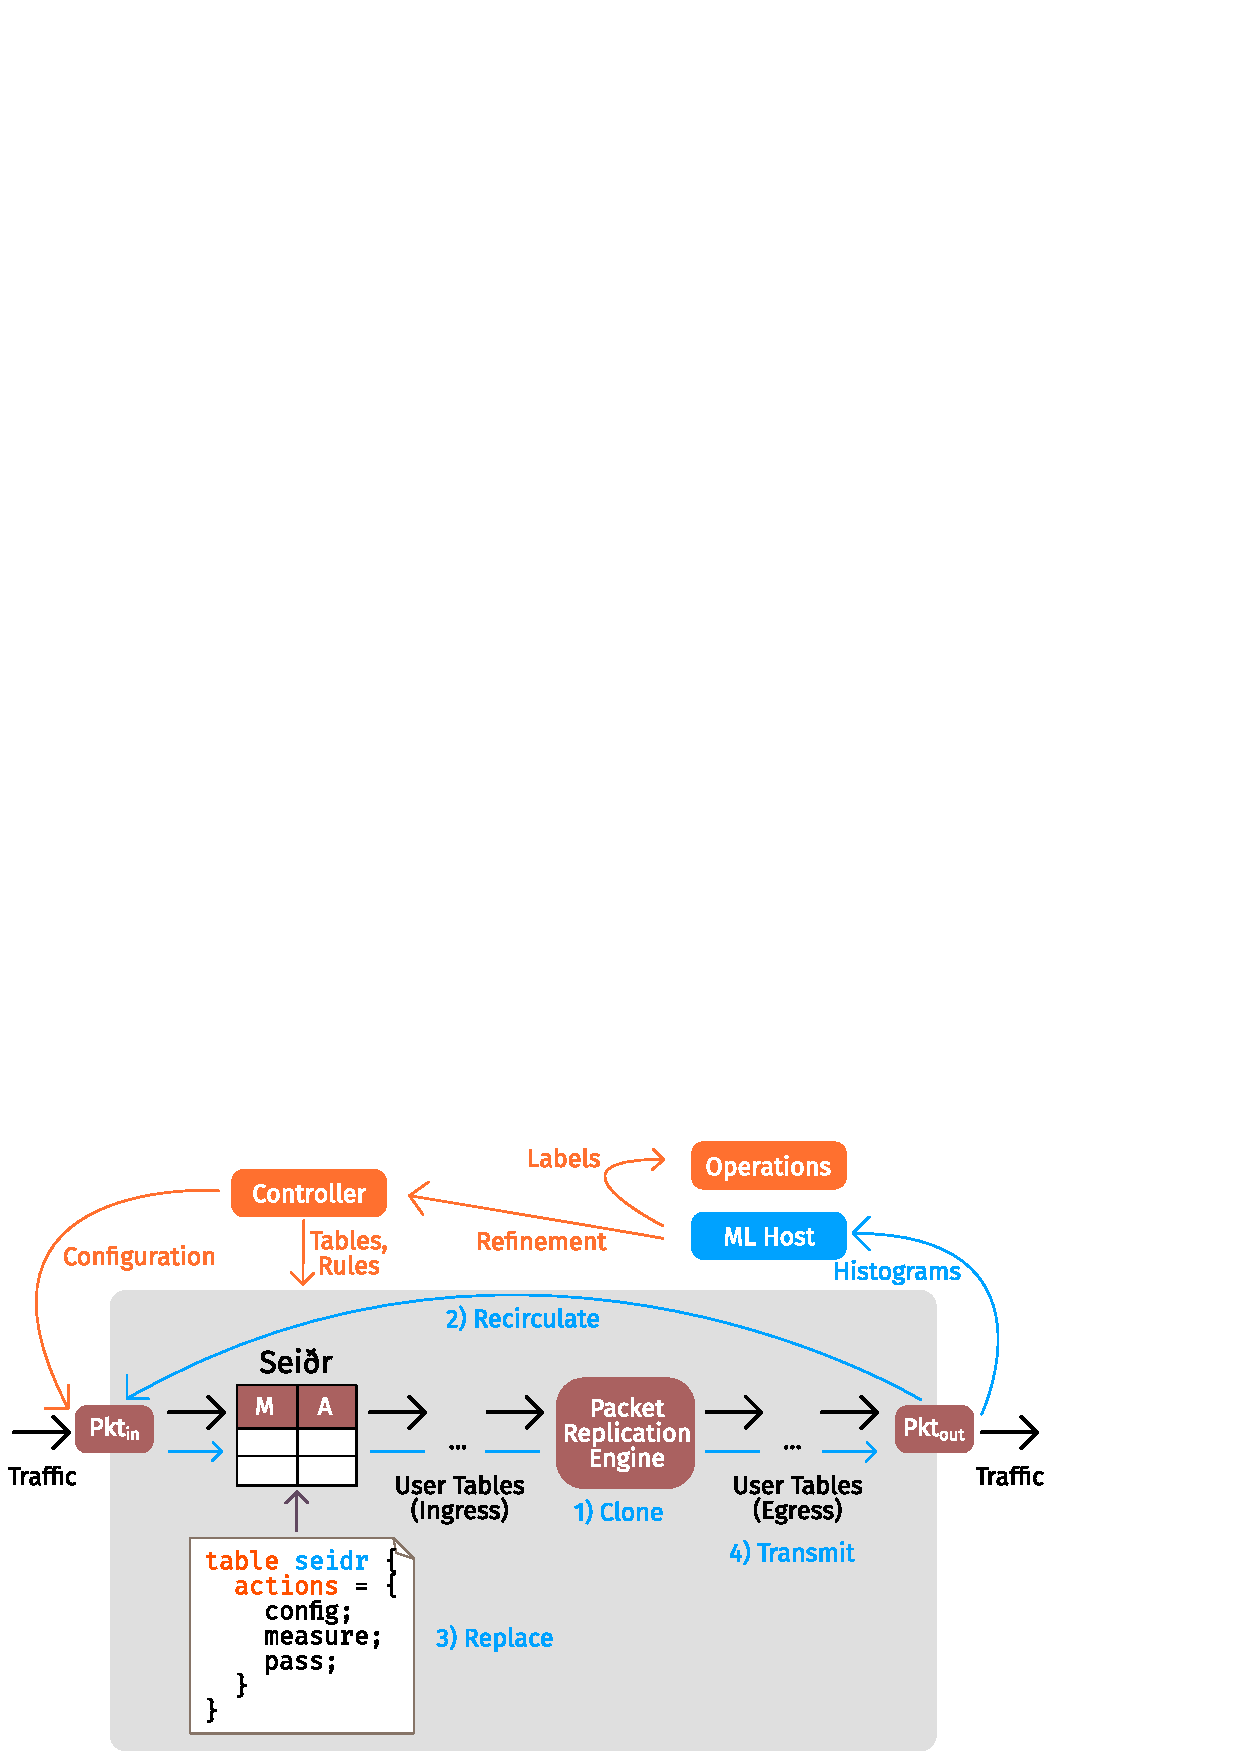
\includegraphics{diagrams/seidr/dp-arch-diagram.pdf}}
    \caption[\seidr{}'s integration with a PSA-compatible dataplane.]{\seidr{}'s integration with a \gls{acr:psa}-compatible dataplane, without the use of digest \texttt{extern}s. \seidr{} uses a register block to store many histograms, each comprised of a fixed bucket count. The main \seidr{} table is used to select which flows or packets are tracked and used in the histogram process, allowing runtime control over monitoring via the control plane. When not using digests to emit telemetry (i.e., for transmission over the control plane), we must rewrite and modify cloned packets to contain the histograms---shown in blue.}
    \label{fig:arch}
\end{figure}

% Let's show them a histogram datastructure would look like purely with registers and how would a P4 action populate it - pseudocode or P4 snippet would be nice.
%\sidenote{?? FIGURE::: Can I redo this diagram to show the possibility of digest?}
Although packet timing information is useful in understanding network and flow behaviour, without volume or packet rate reduction it's prohibitively expensive for hosts to handle each packet.
Histogramming acts as the \emph{aggregation step} which makes this class of analysis feasible in high-speed networks.
\Cref{fig:arch} demonstrates how \seidr{}, installed as an additional table in any P4 program, records and transmits inter-arrival time histograms.
The format for these histogram packets is outlined in \cref{fig:seidr-headers}; bucket counts and size are fixed at compile time.
I choose here to store individual buckets as \mintinline{rust}{u16}s, and fix the number of buckets to \num{100} per histogram as an example (and in later evaluation).
Packets traverse a table which requires \num{3} actions to be implemented:
\begin{enumerate}
    \item \texttt{config} reads any matched packets as a \texttt{seidr\_cfg\_t} of type \texttt{SET\_}\{ \texttt{MIN}, \texttt{MAX}, \texttt{DST}, \texttt{SRC}, \texttt{LEN} \} by using the P4 parser.
    These update registers \numrange{1}{5} in \cref{tab:registers}, dropping any matched packets.
    
    \item \texttt{measure} calculates the inter-arrival time, update per-flow histograms, and transmits finished histograms to the correct host. I describe its operation in \cref{alg:measure}.
    
    \item \texttt{pass} ignores packets, and is the default action.
\end{enumerate}
Constructing \seidr{} in this manner allows the control plane to install rules to enable or disable runtime reconfiguration as needed, and to monitor as many or as few flows as desired (\ie, using wildcard rules or exact matching).

\begin{figure}
\centering
\begin{subfigure}{0.45\linewidth}
\centering
\adjustbox{max width =\linewidth}{
\begin{minipage}{\linewidth}
\begin{minted}[escapeinside=||]{rust}
|\textbf{\textcolor{Keyword}{header}}| seidr_cfg_t {
    bit<8> function;
    bit<144> payload;
}
\end{minted}
\end{minipage}
}
\end{subfigure}
\begin{subfigure}{0.45\linewidth}
\centering
\adjustbox{max width =\linewidth}{
\begin{minipage}{\linewidth}
\begin{minted}[escapeinside=||]{rust}
|\textbf{\textcolor{Keyword}{header}}| seidr_t {
    bit<128> src_ip;
    bit<128> dst_ip;
    bit<16> src_port;
    bit<16> dst_port;
    bit<16> eth_type;
    bit<BUCKETS * 16> histo;
}
\end{minted}
\end{minipage}
}
\end{subfigure}
\caption{P4 headers for \seidr{} configuration and histograms.}\label{fig:seidr-headers}
\end{figure}

\begin{algorithm}
% \vspace{-0.25cm}
% \DontPrintSemicolon
\KwData{5-tuple, P4 metadata, P4 headers, Registers}
h $\leftarrow$ hash(5-tuple)\label{algline:prep-start}\;
index $\leftarrow$ BUCKETS * h\;
owner $\leftarrow$ HistoOwner[h]\label{algline:prep-end}\;
\uIf{metadata.packet\_path = RECIRCULATE}{
    headers.tcp.valid $\leftarrow$ false\label{algline:rewrite-start}\;
    headers.udp.valid $\leftarrow$ true\;
    headers.seidr.valid $\leftarrow$ true\;
    copy 5-tuple into headers.seidr\;
    rewrite headers.ip, headers.udp using HistoSrc/Dest\;
    headers.seidr.histo $\leftarrow$ HistoData[index..]\;
    truncate payload\;
    zero out registers: BucketCount, HistoOwner[h], HistoData[index..]\;\label{algline:rewrite-end}
}
\ElseIf{owner = 0 \textbf{or} owner = 5-tuple}{\label{algline:owner-check}
    HistoOwner[h] $\leftarrow$ 5-tuple\label{algline:iat-prep-start}\;
    iat $\leftarrow$ LastTimestamp[h] - metadata.mac\_ingress\_time\label{algline:iat-prep-end}\;
    \If{iat $\ge$ Min \textbf{and} iat $\le$ Max}{
        bucket $\leftarrow$ BUCKETS * (iat - Min) / (Max - Min)\label{algline:bucket-start}\;
        HistoData[index + bucket] $\leftarrow$ HistoData[index + bucket] + 1\;
        BucketCount[h] $\leftarrow$ BucketCount[h] + 1\label{algline:bucket-end}\;
        \If{BucketCount[h] = Len\label{algline:emitcheck}}{
            mark packet for cloning and recirculation\label{algline:recirc}\;
        }
    }
	LastTimestamp[h] $\leftarrow$ metadata.mac\_ingress\_time\label{algline:update-ts}\;
}

\caption{\seidr{} histogram update and transmission.}\label{alg:measure}
\end{algorithm}

\seidr{}'s operation---\cref{alg:measure}---is generally rather simple.
For now, we will leave aside \crefrange{algline:rewrite-start}{algline:rewrite-end} until \cref{sec:seidr-histo-tx}.
When a flow is to be measured, we first hash its 5-tuple ($h$) and determine which flow is currently occupying slot $h$ (\crefrange{algline:prep-start}{algline:prep-end}).
In the event of hash collision (\cref{algline:owner-check}), we ignore packets outside of the tracked flow to ensure that data is accurate.
As later processing and classification directly affect what decisions are made by operators or automatically taken by a policy (possibly leading to incorrect flow limits, QoS, \emph{etc.}), avoiding corruption/cross-contamination of operational data is paramount.
If the slot is unoccupied or belongs to the current flow, we compute the \gls{acr:iat} and assert ownership over the hash table slot (\crefrange{algline:iat-prep-start}{algline:iat-prep-end}).
Assuming the computed \gls{acr:iat} is within bounds, we compute its bucket index in this interval and increment that bucket and a global counter (\crefrange{algline:bucket-start}{algline:bucket-end})---the global counter triggers a packet emission if it exceeds a known \emph{Len} (\cref{algline:emitcheck}).
Finally, we update the flow's last timestamp (\cref{algline:update-ts}).
To gain collision resistance, \emph{Robin Hood}~\parencite{DBLP:conf/focs/CelisLM85} or \emph{Cuckoo}~\parencite{DBLP:conf/esa/PaghR01} hashing could be used up to a maximum distance in the table, treating a zeroed owner as empty and an illegal source \gls{acr:ip} address as a tombstone value.

\begin{table}
    \centering
    \caption{\seidr{} register map and required sizes using an an $h$-bit hash.}
%    \resizebox{\linewidth}{!}{
    	\expandableinput{tables/seidr/registers}
%    }
    \label{tab:registers}
\end{table}

% Basic Logic:
% \begin{itemize}
%     \item table 1: three actions
%     \begin{itemize}
%         \item config: set R1 or R2 (controller installs rule matching a specific port/ip combo)
%         \item measure: take ingress timestamp from metadata, do stuff, write into lasttime, add to bucket and total if within bounds
%         \item pass (default)
%     \end{itemize}
%     \item then pass onto rest of tables
%     \item Why do it this way? can make it all or nothing through control plane.
%     \item How to write and send packet? Same trick as ESNET? (recirc w/ custom metadata to transform pkt)
% \end{itemize}

% ?? NOTE: See PSA \cite{p4-psa} for register format. Some papers, like Dapper, suggest that hash tables should be possible? That would work out very well in our benefit.

% ?? What is configurable? Min, max of the histogramming range

This design allows runtime configuration of all aspects save for the bucket count; at runtime, the only way to increase bucket resolution is to examine a smaller region of \glspl{acr:iat}.
While in theory this could be configured below a maximum compiled into the firmware, the difficulties introduced by classification and later data processing make this infeasible.
Unless using stream-capable classifiers such as \glspl{acr:lstm}, changing the input size requires retraining from scratch since new neuron weights must be added and structural properties of the input data change.
Increasing the bucket count requires new firmware installation, as many dataplane P4 implementations cannot allocate variable-length stores due to the lack of a dynamic allocator.

\begin{figure}[]
    \centering
    \begin{subfigure}[t]{\linewidth}
        \centering
        \resizebox{\linewidth}{!}{\includegraphics{plots/seidr/dt-cubic-1000-app.pdf}}
        \subcaption{TCP Cubic}
        \label{fig:cubic-hist-app}
    \end{subfigure}

    \begin{subfigure}[t]{\linewidth}
        \centering
        \resizebox{\linewidth}{!}{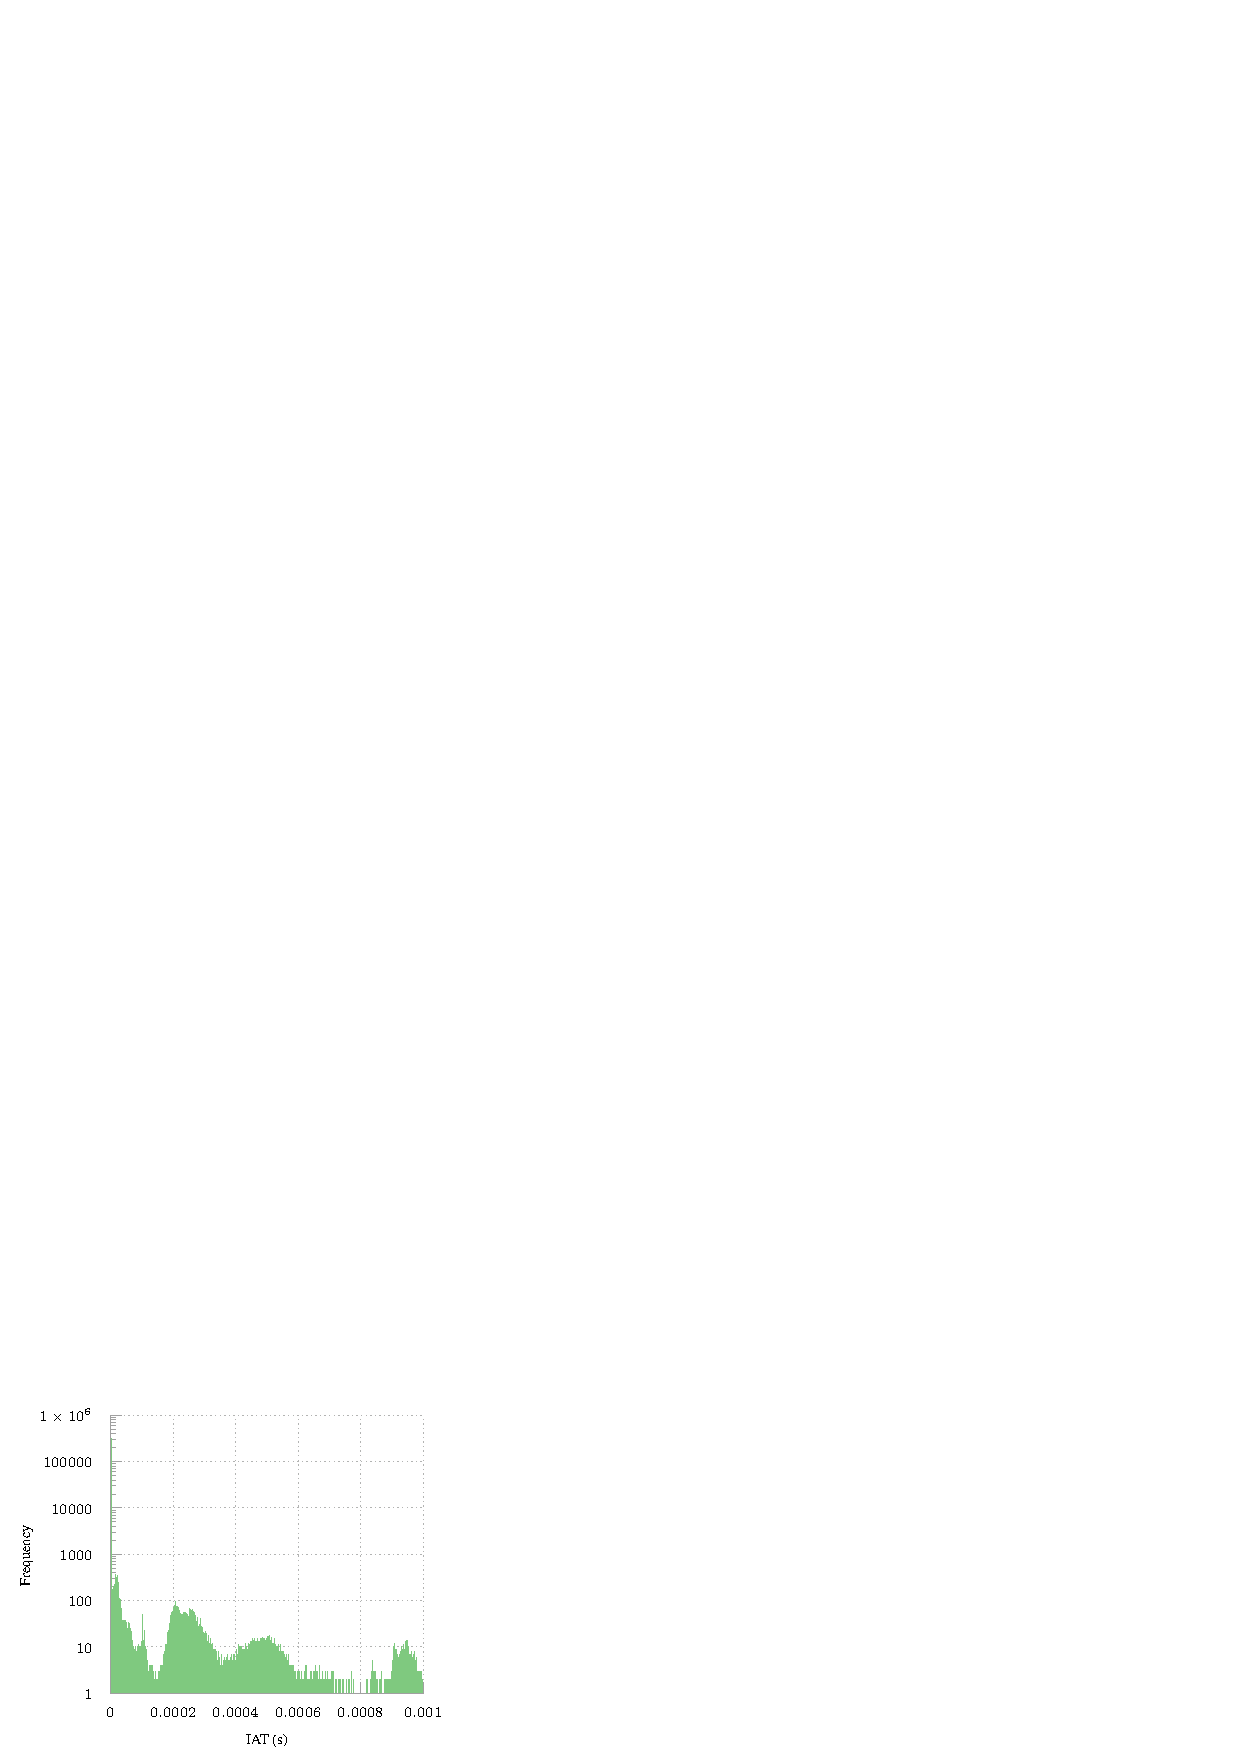
\includegraphics{plots/seidr/dt-bbr-1000-app.pdf}}
        \subcaption{TCP BBR}
        \label{fig:bbr-hist-app}
    \end{subfigure}

    \caption[Example dataplane histograms showing visible differences in inter-arrival times of selected TCP flavours.]{Example dataplane histograms showing visible differences in inter-arrival times of selected \gls{acr:tcp} flavours. These plots examine sub-\qty{1}{\milli\second} dynamics of two separate flows of \qty{1000}{\mega\bit\per\second} traffic generated according to \cref{sec:seidr-datasets}, over these flows' entire lifecycles. BBR flows have significantly more \glspl{acr:iat} measured in the \qtyrange{100}{800}{\micro\second} band, with additional structural differences outside this significant region.}
    \label{fig:tcp-hist-app}
\end{figure}

As a visual example of dataplane-generated histograms, \cref{fig:tcp-hist-app} shows the distribution of inter-arrival times between two \gls{acr:tcp} congestion control algorithms under otherwise identical conditions.
While I cover the underlying causes for these stark differences in more detail later (\cref{sec:seidr-tcpcc}), it should be clear that there are variations in the \emph{distribution} of features that are visible to us (as humans) quite plainly.
It stands to reasons that they should also be visible to a trained \gls{acr:ml} classifier.
%The visible differences are programmatically identified later in \cref{sec:seidr-evaluation} using our \gls{acr:ml} algorithms.
While these particular histograms are taken at the macro level---over the entire lifecycle of a flow---this also gives us cause to look into shorter measured windows.

\subsection{Histogram transmission}\label{sec:seidr-histo-tx}
When targeting the P4-\gls{acr:psa}, we have some options in how histograms may be transmitted from the \gls{acr:pdp} hardware of interest---either to the control plane or dataplane.
If we choose to emit histogram packets to the control plane, we may make use of \emph{digest} \texttt{extern}s which are offered by many \gls{acr:psa}-compliant devices (though aren't strictly required).
Practically speaking, these allow us to pack and emit arbitrary \texttt{struct}s which are delivered to the attached controller \gls{acr:cpu} over the P4Runtime \gls{acr:api}.

\Cref{alg:measure,fig:arch} instead show a more complex case, where we emit generated histogram packets in-band on the dataplane.
The \gls{acr:psa} does not have any explicit mechanisms for generating new packets to be carried by the \emph{dataplane}.
To circumvent this, any packet which would complete a histogram is tagged for cloning at the end of the ingress pipeline, and recirculation at egress (\cref{algline:recirc}).
This truncated copy returns to \seidr{}'s table, where we enable the relevant headers, change L2/3 fields, and write out the histogram contents (\crefrange{algline:rewrite-start}{algline:rewrite-end}).
The P4 deparser outputs the new protocol stack at egress, and transmits the histogram UDP packet into the network.
Although achieved in a somewhat roundabout way, this does have an upside in that it's compatible with the guaranteed core functions of the \gls{acr:psa}.
In future, event-driven architecture proposals~\parencite{DBLP:conf/hotnets/IbanezABM19} may allow first-class support for packet generation.

There are tangible reasons to prefer emitting histograms to the dataplane in spite of the added complexity and recirculations.
Although the data volume and packet-per-second reductions offered by \seidr{} histograms are strong, the former case pushes the steering of all generated packets onto a single controller per switch.
Intuitively, this is expensive and may very well interfere with regular operation of the control plane.
On the other hand, outputting histograms over the dataplane allows administrators to make use of existing \glspl{acr:asic}-backed infrastructure to load-balance classifications across typical host machines.
Alternatively, we might forward packets directly to dedicated, network-connected accelerators like BrainWave whose outputs then inform control plane operation.
Both of these cases spare the control plane of extra load, at modest additional bandwidth cost due to the reduction in telemetry volume.
Digests of course have their own benefits: in some \gls{acr:psa} implementations they may be built in the egress pipeline, adding flexibility for how \seidr{} might be integrated with existing forwarding plane designs (rather than forcing its inclusion in the \emph{ingress} pipeline).

%?? outline benefits and drawbacks of each.
%
%?? talk abt new stuff in heres.
%
%?? Big open qs:
%?? relevance of PSA digests? These can emit packets, no? These can emit an arbitrary struct to the ctl plane over P4Runtime API. Might be good if no digest support, . Digests have a few extra benefits: In some dataplanes can be emitted in egress. Is message fusion a possible downside? (unpredictable)
%?? Maybe 2 options? Can be in-band or out-of-band. Digests are the out-of-band option, meanwhile in-band allows you to use dataplane to forward to accelerators like BrainWave (don't add extra load to ctl plane in this way?)

%?? Header size limits are the other main constraint.
%?? THis is probably not a problem with digests.
%?? WHen emitting to dataplane, however? Will have plat-dependent limits on output. Header size limits, PHV limits, register access reqs that could prevent digest access? Need to mark in-progress histo emissions, progress for each, and emit bitslices spread over multiple egress pkts. Logic: CLONE LOOP WHile still pkts to write, block updates to histo if progress (1 bit?). Limitation: Histo emission freq must be reduced to prevent massive traffic amp. slicing logic could be extended to include the digest case? Are there PHV limits in the digest case that make this really suck?

Another design constraint where these two differ is in header-size limits\sidenote{These designs and implementations again focus on using Netronome \gls{acr:nfp} SmartNICs, as opposed to Tofino \gls{acr:rmt} hardware where such limits do in fact apply.}.
In the case of digests we can assume that a P4 switch is capable of emitting larger packets: following the specification, switches are free to collate generated digests together before handing them off to the control plane.
For transit via the dataplane, however, platform-dependent limits will apply to output packets---particularly as we must use rewritten header fields for this purpose.
This leads to a problem which \cref{alg:measure} does not directly account for: histogram data may be larger than headers allow for.
To fix this, we must make some high-level modifications to its behaviour.
We must mark in-progress transmissions and emit bitslices from the output histogram split over several egress packets by performing a clone loop, where each non-terminal histogram packet is cloned and marches the `send window' forward.
Until termination, updates to the histogram's recorded data are blocked.
A key limitation, however, is that the histogram generation frequency and other parameters must be tuned to prevent traffic amplification driven by the switch.

\subsection{Accurate, precise and high-resolution timestamping}

Precise timestamps are critical when detecting temporal properties of flow behaviour, such as microbursts or inferring flow congestion control algorithms.
It is especially important in high speed (\qty{100}{\giga\bit\per\second}) networks, where there can be as little as \qty{6.7}{\nano\second} between packets that need to be analysed.
With a Linux-based software solution (\eg, reading packets from a link with \emph{tcpdump}), the Linux kernel can only provide microsecond-level accuracy with precision in the order of \qty{100}{\micro\second}~\parencite{DBLP:conf/noms/KundelSBRK20}.
\gls{acr:dpdk} improves on this, increasing the accuracy to \qty{100}{\nano\second} in the best case~\parencite{DBLP:journals/ccr/PrimoracBA17}.
However, today's dataplane devices (\eg, Netronome SmartNICs, NetFPGA SUME) allow nanosecond-accurate timestamps to be retrieved from the \gls{acr:mac} modules with a precision of \qty{10}{\nano\second}~\parencite{DBLP:conf/noms/KundelSBRK20}, a timestamp property \seidr{} relies upon.

% Some platforms provide picosecond-level precision and many solutions allow time synchronisation between multiple devices using the IEEE 1588-2002 (Precision Time Protocol) standard.

